\chapter{Conclusões, Trabalhos Futuros e Cronograma}\label{cap:conclusao} 

Este capítulo abordará as conclusões dessa  proposta de mestrado referentes aos resultados do capítulo \ref{cap:resultados},  bem como uma seção de Trabalhos Futuros e  Cronograma. Na seção de Conclusão serão feitas considerações finais dos resultados de cada base de dados apresentadas, e logo após, em Trabalhos Futuros tem a pretenção de melhorar e expandir tudo que fora realizado  nesta pesquisa, e expor que existe uma continuidade para todo esse estudo aqui elaborado. Já no Cronograma, será criado uma tabela temporal onde esta será divida em meses e tarefas definindo os passos a serem seguidos até a conclusão da dissertação.

\section{Conclusão}\label{cond}
No capítulo \ref{cap:resultados} foi aplicado algoritmos supervisionados em algumas bases de dados a fim de provar se o problema proposto por este  trabalho foi solucionado. Uma vez conhecido o problema, foi executado dois algoritmos supervisionados servindo de amostra para provar que era possível fazer rotulação de dados com estes algoritmos (Naive Bayes e CART), tema deste trabalho. E já identificando alguns trabalhos que já haviam feito rotulação, como \citeonline{LOPES2014}, utilizando algoritmos supervisionados, este estudo demonstra de forma empírica a execução de outros algoritmos com paradigmas diferentes, aos que já foram realizados em pesquisas anteriores. 

Como o cerne da pesquisa é a rotulação de dados foi apresentados dois algoritmos com paradigmas diferentes, e em ambos, suas execuções nas bases de dados resultaram em respostas satisfatórias no âmbito da rotulação. Embora os rótulos encontrados  em cada base de dados não tenham sido totalmente idênticos, tanto um algoritmo como outro mostraram semelhanças em vários rótulos gerados, como exemplo das bases IRIS e GLASS.

O processo de rotulação é composto por um, ou vários atributos, de maior relevância entre eles junto com sua(s) faixa(s) de valor(es) que mais se repetem, contéudo já visto na subseção \ref{cap:ferramentas:ssec:rotulacao}. Seguindo esse modelo foram adicionadas a cada resultado tabelas mostrando em porcentagem o grau de correlacionamento entre os atributos. A importância desta informação é passar o comportamento destes atributos adquirindo uma idéia geral da correlação entre eles na escolha do atributo rótulo.

No modelo de resolução proposto foi inicialmente utilizado na base de dados Seeds, seção \ref{cap:resultados:ssec:seed:nb}, o algoritmo Naive Bayes. O atributo escolhido em cada cluster para compor o rótulo foi o que obteve  na tabela \ref{tab:execucoes:seed:nb} o maior valor de porcentagem. Na base de dados IRIS os valores escolhidos como rótulo dos clusters  não ocorreram ambiguidades, portanto não houve necessidade de utilizar a variável ${V}$. Todos os três clusters somente tiveram um atributo cada, compondo o rótulo.

Continuando com a base Seeds, após a escolha do atributo que fará parte do rótulo, o segundo passo é a escolha da faixa de valores do atributo. Essa segunda etapa é dependente totalmente da discretização\footnote{seção ~\ref{cap:refTeor:sec:discret}} e independente da primeira etapa. O método é capaz de gerar a faixa de maior repetição de valores de qualquer atributo, mas aqui neste trabalho o que importa é a faixa do atributo rótulo. Para ter mais  confiabilidade  no rótulo o método escolhe a faixa de valores que mais se repetem. No caso desse algoritmo o resultado na tabela \ref{tab:rot:seeds:nb} consegue provar uma boa eficiência, pois em cada 70 elementos do cluster 1, somente 14, ficaram de fora dessa faixa. No cluster 2, somando os dois atributos rótulos tem-se 12 elementos que não estão dentro da representatividade do rótulo. Outro valor pequeno em relação aos 70 elementos. E no cluster 3, somente 5 elementos não estão dentro da faixa considerada rótulo.


\begin{figure}[h!]
    \centering
    \subfloat[Naive Bayes]{
        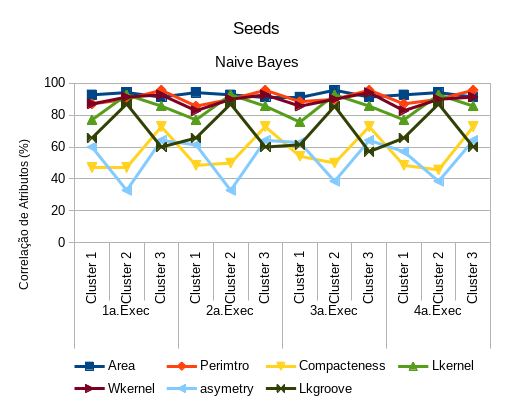
\includegraphics[scale=.8]{figs/grafico_NB_SEED_exec_grp.png}
        \label{fig:execucoes:nb} }
    \quad
    \subfloat[CART]{
        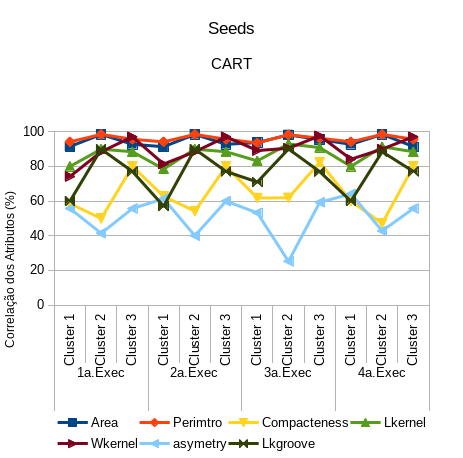
\includegraphics[scale=.8]{figs/grafico_CART_SEED_exec_grp.png}
        \label{fig:execucoes:cart} }
    
    \caption{Gráfico de Execuções dos algoritmos supervisionados na base de dados SEEDS.} \label{fig:graf:SEED_NB_CART}
        
        %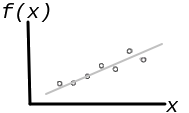
\includegraphics[scale=0.4]{figs/grafB.png}
        %\caption{Polinômio Superajustado} \label{grafB}
\end{figure}


No cenário da execução do algoritmo CART, os resultados foram diferentes dos  apresentados pelo Naive Bayes, mas nem por isso foram insatisfatórios. Contudo uma breve análise sobre as execuções das tabelas ~\ref{tab:execucoes:seed:nb} e \ref{tab:execucoes:seed:cart} podem ser observadas nos gráficos da figura  \ref{fig:graf:SEED_NB_CART}. Como já comentado anteriormente o comportamento dos valores do correlacionamento dos atributos ao longo das execuções mostra-se equilibrada, figura \ref{fig:execucoes:cart}. O gráfico do CART tem um movimento semelhante ao do aplicado do Naive Bayes (figura \ref{fig:execucoes:nb}), embora a variável \textbf{asymetry} saia um pouco do padrão, mas como seus valores são baixos, nada alterou nos rótulos, contudo  o valor de \textbf{perimetro} ficou bastante encostado ao valor da \textbf{area}, fazendo o rótulo \textbf{perimetro} aparecer nos grupos 1 e 2. E também só não foi escolhido pelo grupo 3 , pois  a variável \textbf{Wkernel} estava com valor mais alto. E no gráfico percebe-se que  \textbf{Wkernel} mantém valores altos em todas as execuções do grupo 3.

De acordo com o exposto no parágrafo anterior pode-se dizer sobre análise, que o Naive Bayes acabou tendo resultados um pouco melhores, pois no que diz respeito ao número de elementos fora da faixa definida pelo rótulo, o CART acabou por ter mais elementos fora da faixa de rótulo comparado aos resultados do Naive Bayes. Isso implica dizer que o rótulo deixa de representar mais elementos usando o CART ao invés do Naive Bayes, em outras palavras, o Naive Bayes representou mais elementos concordante com o rótulo do que o CART.


\begin{figure}[h!]
    \centering
    \subfloat[Naive Bayes]{
        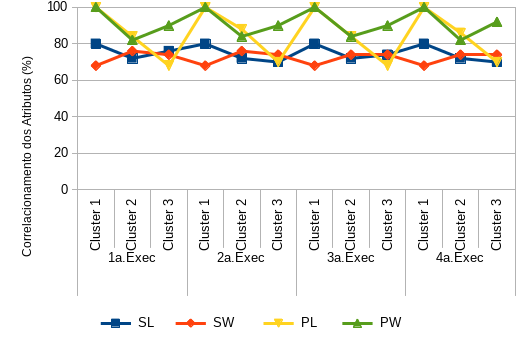
\includegraphics[scale=.9]{figs/grafico_NB_IRIS_exec_grp.png}
        \label{fig:graf:IRIS_NB} }
    \quad
    \subfloat[CART]{
        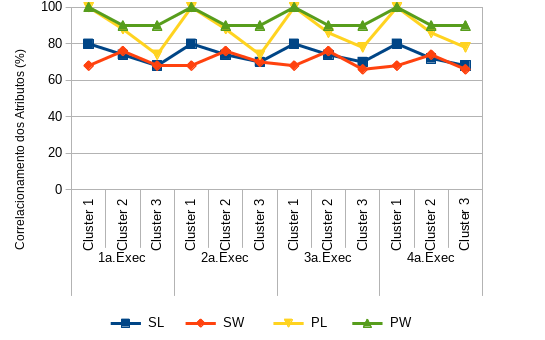
\includegraphics[scale=.9]{figs/grafico_CART_IRIS_exec_grp.png}
        \label{fig:graf:IRIS_CART} }
    
    \caption{Gráfico de Execuções dos algoritmos supervisionados na base de dados IRIS.} \label{fig:graf:IRIS_NB_CART}
        
        %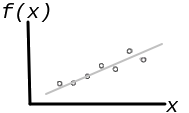
\includegraphics[scale=0.4]{figs/grafB.png}
        %\caption{Polinômio Superajustado} \label{grafB}
\end{figure}

Já na base de dados IRIS, os dois algoritmos supervisionados testados apresentaram os mesmos rótulos nos clusters 1 e 3. Nos gráficos da figura \ref{fig:graf:IRIS_NB_CART} pode-se acompanhar como os valores dos atributos se comportam em seus clusters nas quatro execuções.

Os algoritmos aplicados na base IRIS tem resultados nos gráficos bastantes semelhantes ao da base SEEDS, e logo percebe-se que a base IRIS contêm características que possuem mais atributos bem correlacionados em relação ao da base SEEDS, pois nenhum atributo possui valor abaixo da linha 65(\%) de relacionamento entre eles. Embora no gráfico as  linhas referentes aos comportamentos dos atributos  nos clusters 1 e 3 não sejam totalmentes iguais em cada figura (\ref{fig:graf:IRIS_NB} e \ref{fig:graf:IRIS_CART}), não  modificou o resultado dos rótulos como resposta.

Conforme resultados das tabelas \ref{tab:rot:iris:nb} e \ref{tab:rot:iris:cart} aprensentadas pela execução dos dois algoritmos os rótulos escolhidos no cluster 1 foram dois atributos: \textbf{petalwidth} e  \textbf{petallength}. Onde cada um deles definiram faixas de valor que foi possível abranger 100\% dos elementos. Já no cluster 2 cada algoritmo teve um atributo rótulo diferente, e embora não tivesse a mesma acurácia do cluster 1, obteve um total, de 86\% de acurácia e deixando de representar 7 elementos do rótulo \textbf{petallength} pelo Naive Bayes, e 84\% de acurácia deixando de representar 8 elementos do rótulo \textbf{petalwidth} com CART. E no cluster 3 o atributo escolhido para compor o rótulo foi o \textbf{petalwidth} em ambos os algoritmos. Logo percebe-se a importância do atributo rótulo no cluster 3,  pois o rótulo representa 45 elementos no total de 50 dentro do cluster, deixando somente 5 elementos fora dessa faixa representada pelo rótulo.

%A repetição do atributo \textbf{petalwidth} em todos os rótulos, acaba mostrando o grau de relevância desse atributo na base de dados. Para um especialista é interessante saber que esse atributo possue um grande referencial na base de dados. Nos rótulos esse atributo assumiu faixas diferentes conseguindo assim o método da um significado ao cluster. 


\begin{figure}[h!]
    \centering
    \subfloat[Naive Bayes]{
        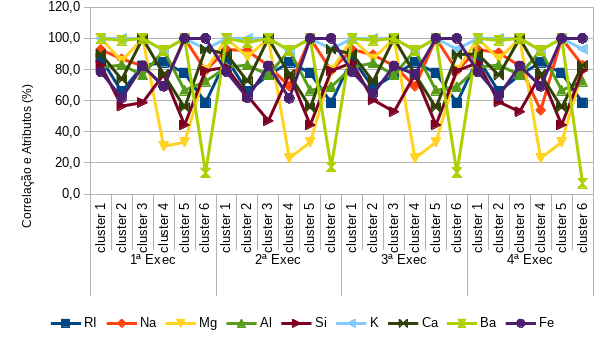
\includegraphics[scale=.9]{figs/grafico_NB_Glass_exec_grp.png}
        \label{fig:graf:GLASS_NB} }
    \quad
    \subfloat[CART]{
        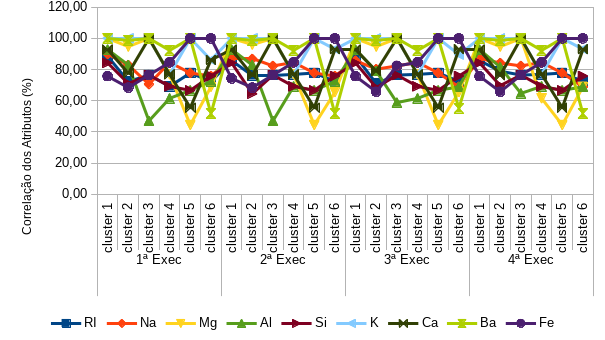
\includegraphics[scale=.9]{figs/grafico_CART_GLASS_exec_grp.png}
        \label{fig:graf:GLASS_CART} }
    
    \caption{Gráfico de Execuções dos algoritmos supervisionados na base de dados GLASS.} \label{fig:graf:GLASS_NB_CART}
        
        %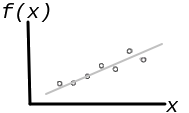
\includegraphics[scale=0.4]{figs/grafB.png}
        %\caption{Polinômio Superajustado} \label{grafB}
\end{figure}

A avaliação da base de dados GLASS referente a rotulação apresentada na tabela \ref{tab:rot:glass:nb} do Naive Bayes, não foi tão bem sucedida quanto ao CART. Dos seis clusters definidos na rotulação somente dois deles não tiveram 100\% de acurácia, e dentre esses dois clusters foi onde obtiveram os mais baixos valores de acurácia.

No cluster 4 em comparação aos dois algoritmos testados, houve umadiferença no Naive Bayes por apresentar três atributos compondo o rótulo, como pode ser visto na tabela \ref{tab:execucoes:glass:nb}, diferente do algoritmo CART que apresentou somente um atributo - \textbf{Ba} - também presente no rótulo do Naive Bayesno. No CART por aprensetar somente um atributo com sua faixa, acabou mitigando o erro e obtendo uma maior porcentagem de acurácia.

Nos gráficos da figura \ref{fig:graf:GLASS_NB_CART} é aprensentado o comportamento de correlacionamento dos atributos rótulos do Naive Bayes e CART respectivamente, e mesmo havendo semelhança nos gráficos os valores de correlação dos atributos no CART foram melhores, e por conseguinte teve melhor acurácia comprovado no gráfico \ref{fig:graf:grafico_NB_CART_acuracia}.

Por fim, ao se analisar os resultados nos dois algoritmos supervisionados pode-se afirmar que  foram bem satisfatórios nas bases utilizadas, conforme figura \ref{fig:graf:grafico_NB_CART_acuracia}, que mostra uma acurácia de 80\% na maioria dos resultados e desta maneira provando que é possível a rotulação de dados com Naive Bayes e CART, portanto os rótulos encontrados representam bem os clusters testados. %E uma obsevação técnica dos algoritmos utilizados é que o CART se mostrou bem mais rápido em relação ao Naive Bayes para gerar os resultados.

\begin{figure}[h!]
    \centering
  %  \subfloat[Naive Bayes]{
  %      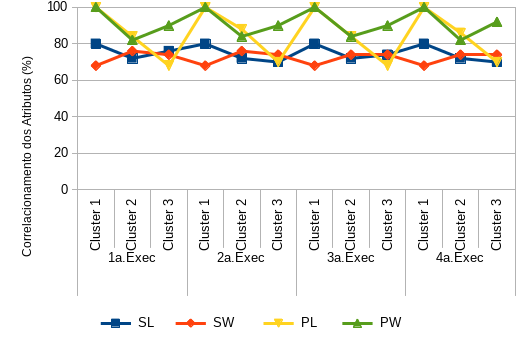
\includegraphics[scale=0.8]{figs/grafico_NB_IRIS_exec_grp.png}
  %      \label{fig:graf:IRIS_NB} }
  %  \quad
  %  \subfloat[CART]{
  %      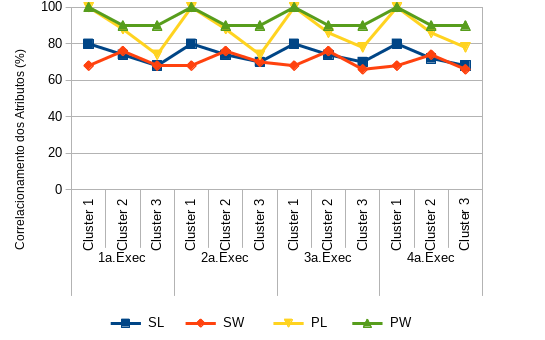
\includegraphics[scale=0.9]{figs/grafico_CART_IRIS_exec_grp.png}
  %      \label{fig:graf:IRIS_CART} }
  %  
  %  \caption{Gráfico de Execuções dos algoritmos supervisionados na base de dados IRIS.} \label{fig:graf:IRIS_NB_CART}
        
  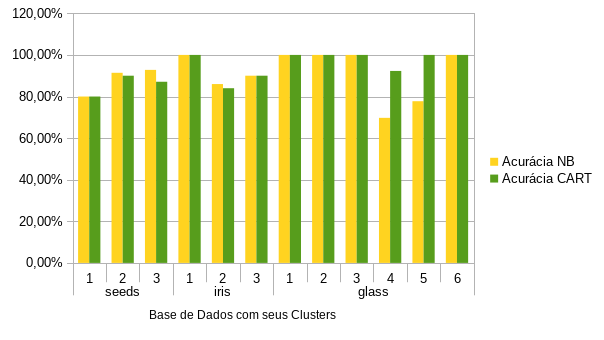
\includegraphics[scale=1]{figs/grafico_NB_CART_acuracia.png}
  \caption{Acurácia por Clusters (Os clusters estão numerados em ordem crescente em cada Base de Dados} \label{fig:graf:grafico_NB_CART_acuracia}
\end{figure}





%\section*{Trabalhos Futuros}
%\addcontentsline{toc}{chapter}{Trabalhos Futuros}
\section{Trabalhos Futuros}\label{cap:fut}

A pesquisa ainda precisa de mais divulgação na esfera acadêmica, e para isso a publicação de um artigo sobre os resultados apresentados aqui é uma consolidação dessa proposta de mestrado já voltada para a dissertação propriamente dita.

Fazer testes com mais bases de dados  provando que esse método pode ser utilizado em várias bases com características  diferentes.
%Fazer testes com mais bases de dados  e com isso traçar uma estratégia caso seja necessário a utilização da idéia de rotulação por algum fim. Caso algum órgão/setor/empresa precise utilizar a rotulação em seu meio, seria interessante o analista de dados,  saber com quais algoritmos supervisionados ele obteria melhores resultados. Embora se saiba nesse estudo que quaisquer algoritmos supervisionados são capazes de realizar a rotulação de dados, também foi provado que em algumas bases um algoritmo se sobressai a outro. Por consequencia disso ter um maior número de base com características diferentes ajudaria em uma tomada de decisão.

Outro ponto importante é inserir nos teste mais algoritmos, que pertençam a  paradigmas diferentes dos que já foram utilizados.

%* de acordo com autor PEARSON, onde os paradigmas são divididos em :  ...... pode-se perceber que existe uma proximidade na afirmação de rotulação para quaisquer algoritmo supervisionado, não sendo ainda possível afirmar esse tema, por falta de testes em alguns algoritmos de paradigmas ainda não testados, mas já deixando par atrabalhos futuros



%\section*{Cronograma}
%\addcontentsline{toc}{chapter}{Cronograma}
\section{Cronograma}\label{cap:cron}

\definecolor{midgray}{gray}{.8}
\begin{table}[!htbp]
\caption{Cronograma de atividades}     % mude aqui para seu título da tabela
\begin{center}

% %  \resizebox{\textwidth}{!}{ % abre resizebox, setar tabela da largura da página.

\scalebox{1}{
\begin{tabular}{p{6cm}lllcc}
\hline
\multicolumn{1}{c}{\multirow{2}{*}{Atividades}} & \multicolumn{5}{c}{Meses} \\ \cline{2-6}
\multicolumn{1}{c}{} & Maio & Junho & Julho & Agosto & Setembro   \\ \hline \hline
%\rowcolor[HTML]{EFEFEF}
\footnotesize Testes com Novas Bases de Dados  & \cellcolor{midgray} ~~~~~~~~~ & \cellcolor{midgray} ~~~~~~~~~ & ~~~~~~~~~ & ~~~~~~~~~ & ~~~~~~~~~  \\ \hline
\footnotesize Modificar Números de Faixa (R) & \cellcolor{midgray} ~~~~~~~~~ & ~~~~~~~~~ & ~~~~~~~~~ &~~~~~~~~~ & ~~~~~~~~~ \\ \hline
\footnotesize Testar com outros Métodos de Discretização & \cellcolor{midgray}~~~~~~~~~ & \cellcolor{midgray}~~~~~~~~~ & ~~~~~~~~~ & ~~~~~~~~~ & ~~~~~~~~~ \\ \hline
\footnotesize Testar com outros Algoritmos com Paradigmas Diferentes &~~~~~~~~~ & \cellcolor{midgray} ~~~~~~~~~ & \cellcolor{midgray} ~~~~~~~~~ & ~~~~~~~~~ & ~~~~~~~~~ \\ \hline
\footnotesize Preparar Artigo   & ~~~~~~~~~ & ~~~~~~~~~ & ~~~~~~~~~ & \cellcolor{midgray} ~~~~~~~~~ & \cellcolor{midgray}  ~~~~~~~~~ \\ \hline
\footnotesize Escrita da Dissertação & ~~~~~~~~~  & \cellcolor{midgray}~~~~~~~~~ & \cellcolor{midgray}~~~~~~~~~ & \cellcolor{midgray} ~~~~~~~~~ & \cellcolor{midgray} ~~~~~~~~~ \\ \hline
\hline
\end{tabular}
} % fecha resizebox
\end{center}
\label{cronograma} % para referencia no texto.
\end{table}


